\documentclass[a4paper]{article}

\usepackage[romanian]{babel}
\usepackage{amsmath}
\usepackage{indentfirst} % indenteaza primul paragraf din fiecare sectiune
\usepackage{graphicx}
\usepackage{hyperref}
\usepackage{caption}
\usepackage{subcaption} % pentru subfiguri
\usepackage{enumitem}

\renewcommand{\phi}{\varphi} % use phi from amsmath
\renewcommand{\Omega}{\varOmega} % use Omega from amsmath

\title{Referat: Experiența Debye-Scherrer de difracție a electronilor pe o rețea
policristalină}
\author{Nicolas Dumitru}

\begin{document}

\maketitle

\section{Scopul lucrării}
\begin{itemize}
	\item Determinarea lungimii de undă asociată electronilor
	\item Verificarea ecuaţiei de Broglie
	\item Determinarea constantelor de reţea ale grafitului
\end{itemize}

\section{Teoria lucrării}
Lungimea de undă a undei asociate unei particule libere e dată de relația
\begin{equation} \label{eq:particle_wavelength}
	\lambda = \frac{h}{p}
\end{equation}
unde $p$ este impulsul particulei și $h$ este constanta lui Planck

Energia unui electron accelerat de o diferenţă de potenţial (tensiune) este
\begin{equation} \label{eq:electron_energy}
	e U = \frac{p^2}{2 m}
\end{equation}
unde \begin{description}
	\item $U$ --- tensiunea de accelerare
	\item $e$ --- sarcina electronului
	\item $p$ --- impulsul electronului
\end{description}

Din ecuația \eqref{eq:electron_energy} obținem $p = \sqrt{2 m e U}$, iar din
\eqref{eq:particle_wavelength} rezultă
\begin{equation} \label{eq:lambda_U}
	\lambda = \frac{h}{\sqrt{2 m e U}} \text{,}
\end{equation}
ceea ce arată că lungimea de undă $\lambda$ depinde de tensiunea de accelerare
$U$.

Dacă pe un set de plane cristaline paralele cade un fascicul monocromatic de
raze X sau electroni monoenergetici care se presupune că au caracter
ondulatoriu, fiecare element al planului cristalin acționează ca un centru de
împrăștiere generând o undă sferică elementară reflectată, suprapunerea acestor
unde sferice elementare generând un front de undă reflectat. Conform legilor
reflexiei, lungimea de undă a undei reflectate este aceeaşi cu a undei incidente
si unghiul de reflexiei este egal cu unghiul de incidență. Din suprapunerea
undelor reflectate pe plane succesive se obțin maxime de interferență
(interferență constructivă) dacă diferența de drum $\Delta = \Delta_1 + \Delta_2
	= 2 d \sin \theta$ este un multiplu întreg de lungimi de undă:
\begin{equation} \label{eq:Bragg}
	2 d \sin \theta = n \lambda, n = 1, 2, 3, \dots
\end{equation}
unde
\begin{description}
	\item $d$ --- distanța dintre două plane succesive
	\item $\theta$ --- unghiul de incidență măsurat față de plan
\end{description}

Condiția \eqref{eq:Bragg} este cunoscută ca relația Bragg.

Din \ref{fig:difrac_Debye-Scherrer} se obține relația
\begin{equation}
	\tan(2 \theta) = \frac{D}{2 L}
\end{equation}
\begin{description}
	\item $D$ --- diametrul unui inel
	\item $L$ --- distanța de la probă la ecran
\end{description}

Pentru unghiuri $\theta$ mici:
\begin{equation} \label{eq:theta_mic}
	\tan(2 \theta) \approx \sin(2 \theta) \approx 2 \sin \theta
\end{equation}

Substituind \eqref{eq:theta_mic} în \eqref{eq:Bragg} se obține, pentru $n = 1$,
expresia pentru lungimea de undă asociată electronilor:
\begin{equation}
	\lambda = d \frac{D}{2L}
\end{equation}

Ținând cont de ecuaţia \eqref{eq:lambda_U} se obține pentru diametrul inelelor
de difracție:
\begin{equation}
	D = k(d) \frac{1}{\sqrt{U}}
\end{equation}
unde
\begin{equation}
	k(d) = \frac{2hL}{d \sqrt{2 m e}}
\end{equation}
este panta dreptei $D = D(\frac{1}{\sqrt{U}}$ și depinde de constanta de rețea $d$.

\section{Schițe și grafice}

\begin{figure}[htbp]
	\centering
	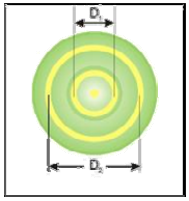
\includegraphics[width=0.3\textwidth]{inele-difractie.png}
	\caption{Reprezentarea schematică a inelelor de difracție. Cele două inele cu
		diametrele $D_1$ și $D_2$ corespund constantelor de rețea $d_1$ și $d_2$.}
\end{figure}

\begin{figure}
	\centering
	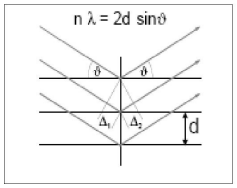
\includegraphics[width=0.3\textwidth]{bragg.png}
	\caption{Reprezentarea schematică a condiției de difracție Bragg}
\end{figure}

\begin{figure}
	\centering
	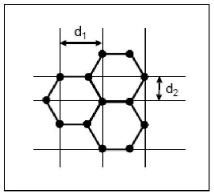
\includegraphics[width=0.3\textwidth]{grafit.png}
	\caption{Constantele de rețea în grafit: $d_1 = 2.13 \cdot 10^{-10} m$;$d_2 = 1.23 \cdot 10^{-10} m$}
\end{figure}

\begin{figure}[htbp]
	\centering
	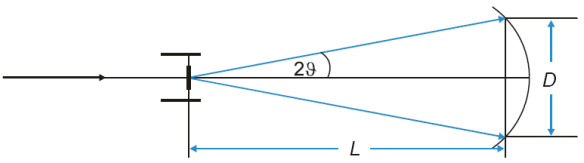
\includegraphics[width=0.3\textwidth]{difractie-debye-scherrer.png}
	\caption{Reprezentarea schematică a difracției Debye-Scherrer \\
		$L = 13.5 cm$ (distanța dintre stratul de grafit și ecran) \\
		$D$ este diametrul inelului de difracție observat pe ecran}
	\label{fig:difrac_Debye-Scherrer}
\end{figure}

\begin{figure}[htbp]
	\centering
	\begin{subfigure}{0.45\textwidth}
		\centering
		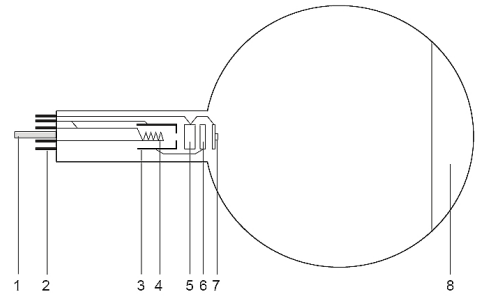
\includegraphics[width=\textwidth]{tub-electronic.png}
		\caption{}
	\end{subfigure}
	\begin{subfigure}{0.45\textwidth}
		\centering
		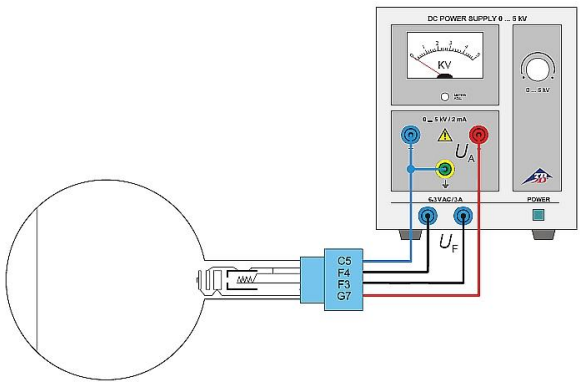
\includegraphics[width=\textwidth]{schema-conexiuni.png}
		\caption{}
	\end{subfigure}
\end{figure}

\end{document}
